\documentclass{article}
\usepackage[a4paper]{geometry}
\usepackage[utf8]{inputenc}
\usepackage{polski}
\usepackage{tabularx}
\usepackage{indentfirst}
\usepackage{multirow}
\usepackage{amssymb}
\usepackage{amsmath}
\usepackage{anysize}
\usepackage{float}
\usepackage{caption}
\usepackage{subcaption}
\usepackage{graphicx}
\usepackage{tikz}
\usepackage{listings}
\usepackage{color}
\usepackage{verbatim}

\usetikzlibrary{shapes}

\definecolor{mygreen}{rgb}{0,0.6,0}
\definecolor{mygray}{rgb}{0.5,0.5,0.5}
\definecolor{mymauve}{rgb}{0.58,0,0.82}

\usepackage{titling}
\newcommand{\subtitle}[1]{%
	\posttitle{%
	\par\end{center}
	\begin{center}\small#1\end{center}
	\vskip0.5em}%
}

\title{Chariot}
\subtitle{Akademia Górniczo-Hutnicza im. Stanisława Staszica w Krakowie\\
	Wydział Elektrotechniki, Automatyki,\\
	Informatyki i Inżynierii Biomedycznej}
\author{Kacper Tonia\and
		Sławomir Kalandyk}
\date{}

\begin{document}
%------------------------------------------------------------
\maketitle

\section{Cel programu}
Zadaniem programu jest rozsyłanie wozów strażackich do~incydentów zgłaszanych za~pośrednictwem strony internetowej. Pula wozów jest ograniczona, zaś same pojazdy po~powrocie z~akcji przez pewien czas pozostają niedostępne (czas na~uzupełnienie zapasów, naprawy itd.).
\section{Moduły}
\begin{itemize}
	\item \textbf{main} -- uruchamia serwer i pełni rolę klienta.
	\item \textbf{central} -- reprezentuje centralę powiadamiania ratunkowego, której można zgłosić żądanie pomocy straży pożarnej. Moduł ten implementuje zachowanie \texttt{gen\_server}.
	\item \textbf{domain} -- definuje rekord \texttt{state} używany przez serwer centrali, a~także tzw.~\emph{invoke functions} -- funkcje realizujące podstawową logikę aplikacji (zapisywanie zgłoszeń, wysyłanie wozów strażackich itd.).
	\item \textbf{firetrucks} -- definiuje rekord \texttt{firetruck} reprezentujący wóz strażacki, a~także podstawowe operacje z~tym rekordem związane.
\end{itemize}

\subsection{Serwer centrali}
Operacje realizowane przez serwer centrali możemy podzielić na~3~kategorie:
\begin{itemize}
	\item operacje opisane przez \texttt{handle\_call} są~synchroniczne, zwracają pewną wartość nie modyfikując stanu serwera.
	\begin{itemize}
		\item \texttt{get\_vehicles} pobiera aktualną listę pojazdów wraz z~ich stanem
	\end{itemize}

	\item operacje opisane przez \texttt{handle\_cast} są~asynchroniczne, nie blokują klienta. Nie zwracają istotnych wartości, ale mogą modyfikować stan serwera.
	\begin{itemize}
		\item \texttt{report\_incident} zgłasza incydent wymagający przyjazdu straży pożarnej
	\end{itemize}

	\item operacje opisane przez \texttt{handle\_info} sygnalizują serwerowi zajście jakiegoś zdarzenia. Nie powinny być wywoływane z~zewnątrz.
	\begin{itemize}
		\item \texttt{report\_enqueued} sygnalizuje, że~w~kolejce zgłoszeń znajdują się oczekujące zgłoszenia
		\item \texttt{dispatch\_finished} sygnalizuje, że~pojazd wrócił z~akcji strażackiej
		\item \texttt{preparation\_finished} sygnalizuje, że~pojazd jest gotowy do~następnej akcji strażackiej
	\end{itemize}
\end{itemize}

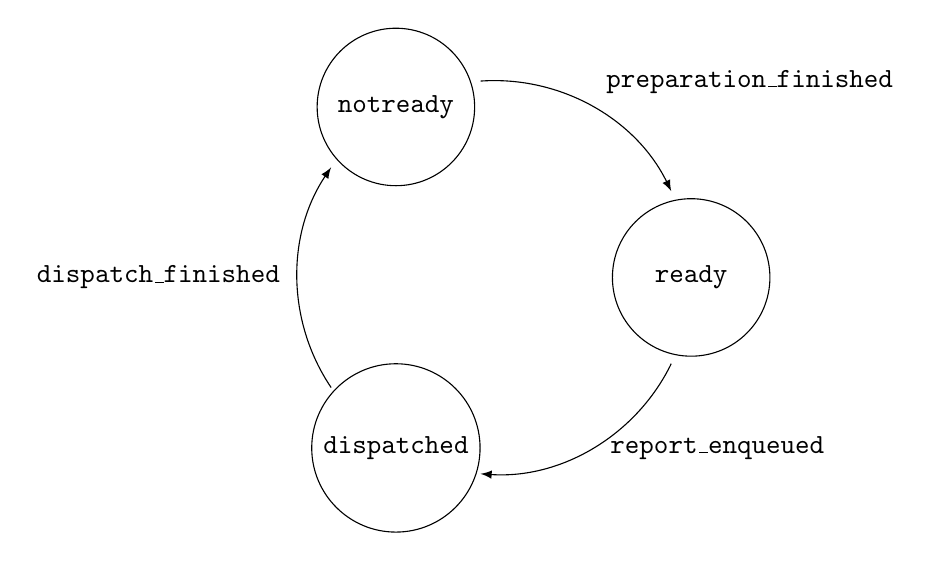
\begin{tikzpicture}[state/.style={circle, draw, minimum size=2cm}]

	\def \n {3}
	\def \radius {2.5cm}
	\def \margin {26} % margin in angles, depends on the radius
	
	\node[state] at (0:\radius) {\texttt{ready}};
	  \draw[<-, >=latex] ({0+\margin}:\radius)
		arc ({\margin}:{360/\n-\margin}:\radius);
	\node at (60:\radius) [above right=0.05cm] {\texttt{preparation\_finished}};
		
	\node[state] at ({ -360/\n }:\radius) {\texttt{dispatched}};
	  \draw[<-, >=latex] ({360/\n+\margin}:\radius)
		arc ({360/\n+\margin}:{360/\n * 2-\margin}:\radius);
	\node at (180:\radius) [left=0.1cm] {\texttt{dispatch\_finished}};
	
	\node[state] at ({ -360/\n * 2 }:\radius) {\texttt{notready}};
	  \draw[<-, >=latex] ({360/\n * 2+\margin}:\radius) 
		arc ({360/\n * 2+\margin}:{360/\n * 3-\margin}:\radius);
	\node at (300:\radius) [right=0.1cm] {\texttt{report\_enqueued}};
	
\end{tikzpicture}

\section{Pakiety zewnętrzne}

\section{Instrukcja obsługi}

\section{Możliwe rozszerzenia programu}

\section{Ograniczenia programu}

\end{document}